\documentclass[../physical_computing.tex]{subfiles}

\begin{document}

\chapter{Starting point}

\section{What is this course?}
\label{sec:whatisit}

A course at University is intended to take the student on a journey between some starting point, a body of knowledge and skills which it is presumed they already have, to some finish point, where the student has learned some new material with some intended purpose. Many courses make the mistake of assuming the starting point is no knowledge at all! This is the safest bet for an academic, but it has two immense disadvantages. First, ignoring the student's existing knowledge means you end up re-teaching material, costing you precious time. Second, the student's existing knowledge may be in some context that they have never questioned. Pointing out that there is a wider world out there that they have not explored may pique their interest and motivate them to devote energy and time to working in your course. An under-appreciated reality of teaching is that it is in part the art of seduction. Students will not work for you unless you can succeed in motivating them to do so.

This course will attempt to raise your enthusiasm level by pointing out that what you probably know about computing is almost certainly confined to an artificial and some would say Utopian environment. Learning how to do computing outside this environment, in the real `physical' world is liberating and fun. Furthermore, many of the applications of computers, or more generally of digital circuits and algorithms, underpin some of the worlds most interesting machines and experiments, from spacecraft to gravitational wave detectors. We will in this course explain the senses in which these statements are true, and we will learn some basic techniques in what I call `physical computing'.

\section{Analysis of a simple program}
\label{sec:projectforstudents}

Most of you will have done a course in computer programming using a high-level language such as PYTHON. Below is a code listing that I lifted from an online programming course for undergraduates.

\begin{minted}{python}
import numpy as np
from matplotlib import pyplot as plt

ys = 200 + np.random.randn(100)
x = [x for x in range(len(ys))]

plt.plot(x, ys, '-')
plt.fill_between(x, ys, 195, where=(ys > 195), \
facecolor='g', alpha=0.6)

plt.title("Sample Visualization")
plt.show()
\end{minted}
The program produces this graphical output.
\begin{figure}[h!]
    \centering
    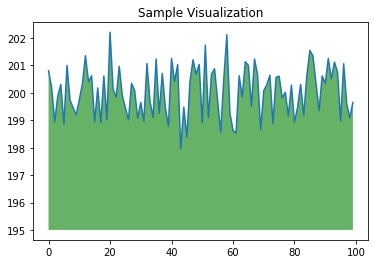
\includegraphics[width=0.8\textwidth]{chapter_1/figures/pythongraph.jpg}
    \caption{Graphical output of the PYTHON program}
    \label{fig:pythongraph}
\end{figure}

Let us analyse this program. First, its job is to make a plot of some random numbers. It probably isn't important exactly how long the code takes to produce this plot, as long as it isn't so long that it could have been done more efficiently without the computer. It also probably isn't critical that the program takes the same amount of time to produce this output every time it is run. 

The program makes use of some imported packages \texttt{numpy} and \texttt{matplotlib}, for mathematical functions and graphical output respectively.
It is somebody else's problem to implement these library functions. The \texttt{matplotlib} plotting function will only work if the computer has a way of outputting graphics. When I ran this code, the graphics appeared in my web browser, but this was because I was using Jupyter notebook; other python environments would have put the graphics in a separate window. 

Other observations about the program might seem obvious, but perhaps only because you have always taken them for granted. First, the program executes by default from top to bottom. Occasionally, there is a command that causes the code to go into a loop, so for example when the values of \texttt{ys} are generated, the
command \texttt{randn} generates 100 random numbers, so this random number 
generator loops around and runs 100 times before the program moves to the next
line of code. Similarly for the next line, which generates 100 values of \texttt{x}. All high-level programming languages feature loops, which cause code to execute multiple times. Another high-level programming concept is a conditional, meaning code that executes under some condition, but not if that condition is not satisifed. Loops and conditionals are so ubiquitous that you take it for granted that programs will utilise them. For that matter, you also take it for granted that code will execute from top to bottom.

Other things you might take for granted are particular to PYTHON. Notice how variables such as \texttt{x}, \texttt{ys} and \texttt{facecolor} represent data of different types, and that the type of data they represent is set automatically by PYTHON when the variables are defined. You don't generally have to declare what type of data a particular variable is going to be set to before that variable is used, PYTHON figures things out on the fly. In this respect, PYTHON differs from other high level languages like C or C++; in those languages you need to DECLARE a variable, including its data type, before you use it. You might think about whether this characteristic of figuring out variable types when they are first used is always a good thing, or whether perhaps it might occasionally cause problems.

The structure of high level computer languages generally comes about from them being intended for programming computers of a particular type. For example, most computers revolve around a very small number of processor cores which do all the calculations. Of course on a modern computer this may be less true than it used to be; there are often many cores on a CPU, and that doesn't include the GPU chip, where there are hundreds or thousands of cores that are more special purpose. In general, however, the architecture we imagine in a computer is that of a processor doing all the calculations, and input data and commands being piped in to this processor in sequence, and output form the processor coming out, so to speak, of the other side.

However, things do not have to be this way. In a more general calculating circuit, you can imagine the input data feeding in to the circuit through multiple parallel paths into a variety of different elements that all do things to subsets of the data at once. Such a circuit could be vastly more efficient than the gridlock that occurs when everything has to be stuffed in to a small number of processor cores. However, there is a price to pay, which is that the calculations in all these elements must be coordinated with each other, so that the outputs of the elements may combined and fed into yet more elements so that more calculations can be done, but on the right numbers. This way of doing things is potentially far more powerful than a conventional single processing unit architecture, but the programming of such a machine is vastly more complex as well. And, consider, the arrangement of the calculating elements for a particular computation may also need to be optimised for the efficiency of that computation. For the next computation, you may want to arrange the circuit differently.

So, in this course, we will consider the construction of digital circuits that do calculations. These circuits are literally wires connecting very fundamental building blocks. Until the 1980s. digital circuits were assembled using literal physical wires or circuit boards, connecting these fundamental blocks together. If you wanted a new circuit, you had to build it out of hardware. In the 1980s, however, large scale integration of digitial hardware led to a more abstract way of doing things. You described the digital circuit that you wanted using a new type of language, a Hardware Description Language (HDL). By a wierd stroke of luck I programmed early circuits of this type, which were called PALs, or programmable arrays of logic, using an early HDL called ABEL, when I was doing work experience at school. I had no idea that I would wind up using it's direct descendent, called VHDL, a far more advanced hardware description language, in my physics research more than 35 years later. Life is strange sometimes. Anyway, the hardware description language literally permits you to build a digital machine. You are building hardware, using a language.

Having built the hardware, in simple cases, you just pipe the data in, and the desired output appears at the other end of your digital machine. This has two great advantages. First, it is extremely fast. There is no operating system or other environment to slpw down the process. Second, often the calculation takes exactly the same amount of time every time it is executed. This makes this type of machine suitable for use in situations where the output of the calculation is used to control the state of something critical, like a physics experiment, where unexpected delays cause glitches which may cause the machine or experiment to stop working.

In more complex cases, your machine may grow to resemble a computer, and you may need to write more code, this time perhaps in a high level language, to program it. But because you have far more control over the architecture of your machine than yo do with an ordinary computer, you are empowered to make a far more interesting, useful and powerful calculation engine. I hope you will enjoy learning physical computing, as I have enjoyed it. It's physics, but not perhaps as you have experienced it before.

\end{document}